\subsubsection{Image Analysis Techniques}
	There are multiple techniques which can be applied to imagery to extract information which include detection of edges or objects and using known data to take measurements. These methods tend to compare data from neighbouring pixels to spot differences which can indicate features.
	\paragraph{Edge Detection}
	This is the application of mathematical algorithms to locate and highlight the edges of features in an image. There are multiple algorithms which can be used for edge detection including Sobel, Roberts, Canny, and fuzzy logic though all utilise the concept of comparing side by side pixel data to find "steps" from one brightness to another.
	\begin{table}[h!]
		\centering
		\caption{Table of pixel data showing an edge}
		\label{tab:edgePixels}
		\begin{tabular}{|c|c|c|c|c|c|c|}
			\hline
			5&7&6&4&152&148&149\\
			\hline
			\cellcolor[HTML]{0D0D0D}&
			\cellcolor[HTML]{121212}&
			\cellcolor[HTML]{0F0F0F}&
			\cellcolor[HTML]{0a0a0a}&
			\cellcolor[HTML]{989898}&
			\cellcolor[HTML]{949494}&
			\cellcolor[HTML]{959595}\\
			\hline
		\end{tabular}
	\end{table}\\
	Table \ref{tab:edgePixels} represents possible pixel values of an edge indicated by the large difference between 4 and 152. The applied algorithm will pick up on this discrepancy and in will be indicated on the resulting image. A common application for edge detection is text recognition such as in automatic number plate recognition (ANPR) \citep{anpr} as the process can remove unwanted background data and highlight the block shapes of the number plate.
	\begin{figure}[h!]
		\centering
		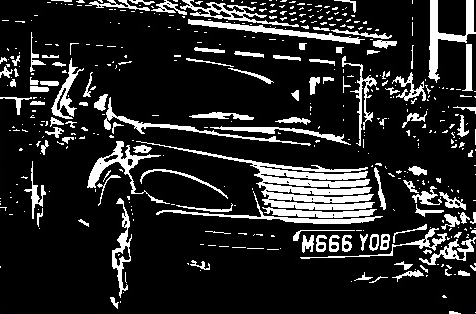
\includegraphics[width=10cm]{../images/anpr.jpg}
		\caption{Edge detection applied to an image for number plate recognition}
		\label{fig:anpr}
	\end{figure} 
	\paragraph{Object Detection}
	Much like edge detection, object detection is used to pick out features in images, the 
	difference being that object is a more abstracted term than edge and could mean anything from 
	faces to signs to company logos. A common technique is Binary Large OBject (BLOB) analysis 
	which is two techniques combined into one application \citep{introtoprocessing}, this includes 
	BLOB extraction which is used to isolate large objects in an image, dismissing small objects as 
	noise, which is then followed by BLOB classification, assigning objects a class based on 
	predetermined parameters.
	\\\\
	Regularly carried out after grayscaling and thresholding an image, BLOB extraction uses a grass-fire algorithm to locate pixels which display a significant difference to the image background and discover the full extent of this region. As all the pixels of each BLOB in a object are known, certain parameters are also known such as size, area, and boundaries. From these parameters, calculations can be carried out to discover the classification of each BLOB, for example with the boundary and area of each BLOB, the circularity can be calculated to locate all the circular objects in an image.
	\begin{equation}
		B_{c}=\frac{B_{p}}{2\sqrt{\pi \times B_{a}}}
	\end{equation}
	\begin{where}
		\item $B_{c}$ is the circularity of the BLOB
		\item $B_{p}$ is the perimeter of the BLOB's bounding box
		\item $B_{a}$ is the area of the BLOB
	\end{where}
	\paragraph{Taking Measurements}
	To measure an object in an image, certain data about the camera and camera's location are 
	required. By using digital imagery the majority of this information is provided as each image 
	contains metadata or EXchangeable Image Format (EXIF) data which includes information such as 
	camera manufacturer, focal length, image size, and location.
	\begin{equation}
		\label{equ:measureobj}
		H_{o} = \Bigg(\frac{f\times\big(\frac{H_{i}}{H_{s}}\big)}{D - f}\Bigg)\times H_{c}
	\end{equation}
	\begin{where}
		\item $f$~~~~is the focal length of the camera lens
		\item $D$~~~is the distance to the object
		\item $H_{o}$~~is the height of the object
		\item $H_{i}$~~is the height of the image in pixels
		\item $H_{s}$~~is the height of the camera sensor
		\item $H_{c}$~~is the height of the camera from the ground
	\end{where}
	\begin{comment}
	\begin{equation}
	\label{equ:measuredist}
		D = \frac{f\times H_{c} \times H_{i}}{H_{o} \times H_{s}}
	\end{equation}
	\begin{where}
		\item $D$~~~is the distance to the object
		\item $f$~~~~is the focal length of the camera lens
		\item $H_{c}$~~is the height of the camera from the ground
		\item $H_{i}$~~is the height of the image in pixels
		\item $H_{o}$~~is the height of the object
		\item $H_{s}$~~is the height of the camera sensor
	\end{where}
	\end{comment}
	\vspace{5mm}
	The process to calculate the height of an object in an image is shown in equation 
	\ref{equ:measureobj}. $f$, $H_{i}$, and $H_{s}$ can be acquired from EXIF 
	data, however $D$ and $H_{c}$ are not collected by the camera and must be measured. When 
	dealing with image analysis this means that this data must have been collected when the image 
	was taken.
	\\\\
	To circumvent the need for this data a reference object of known size can be included in the 
	image, this allows a comparison between the object to be measured and the reference object. The 
	previously mentioned mars rover, Curiosity, carries a United States penny and charts to 
	calibrate its cameras against.
	\begin{figure}[h!]
		\centering
		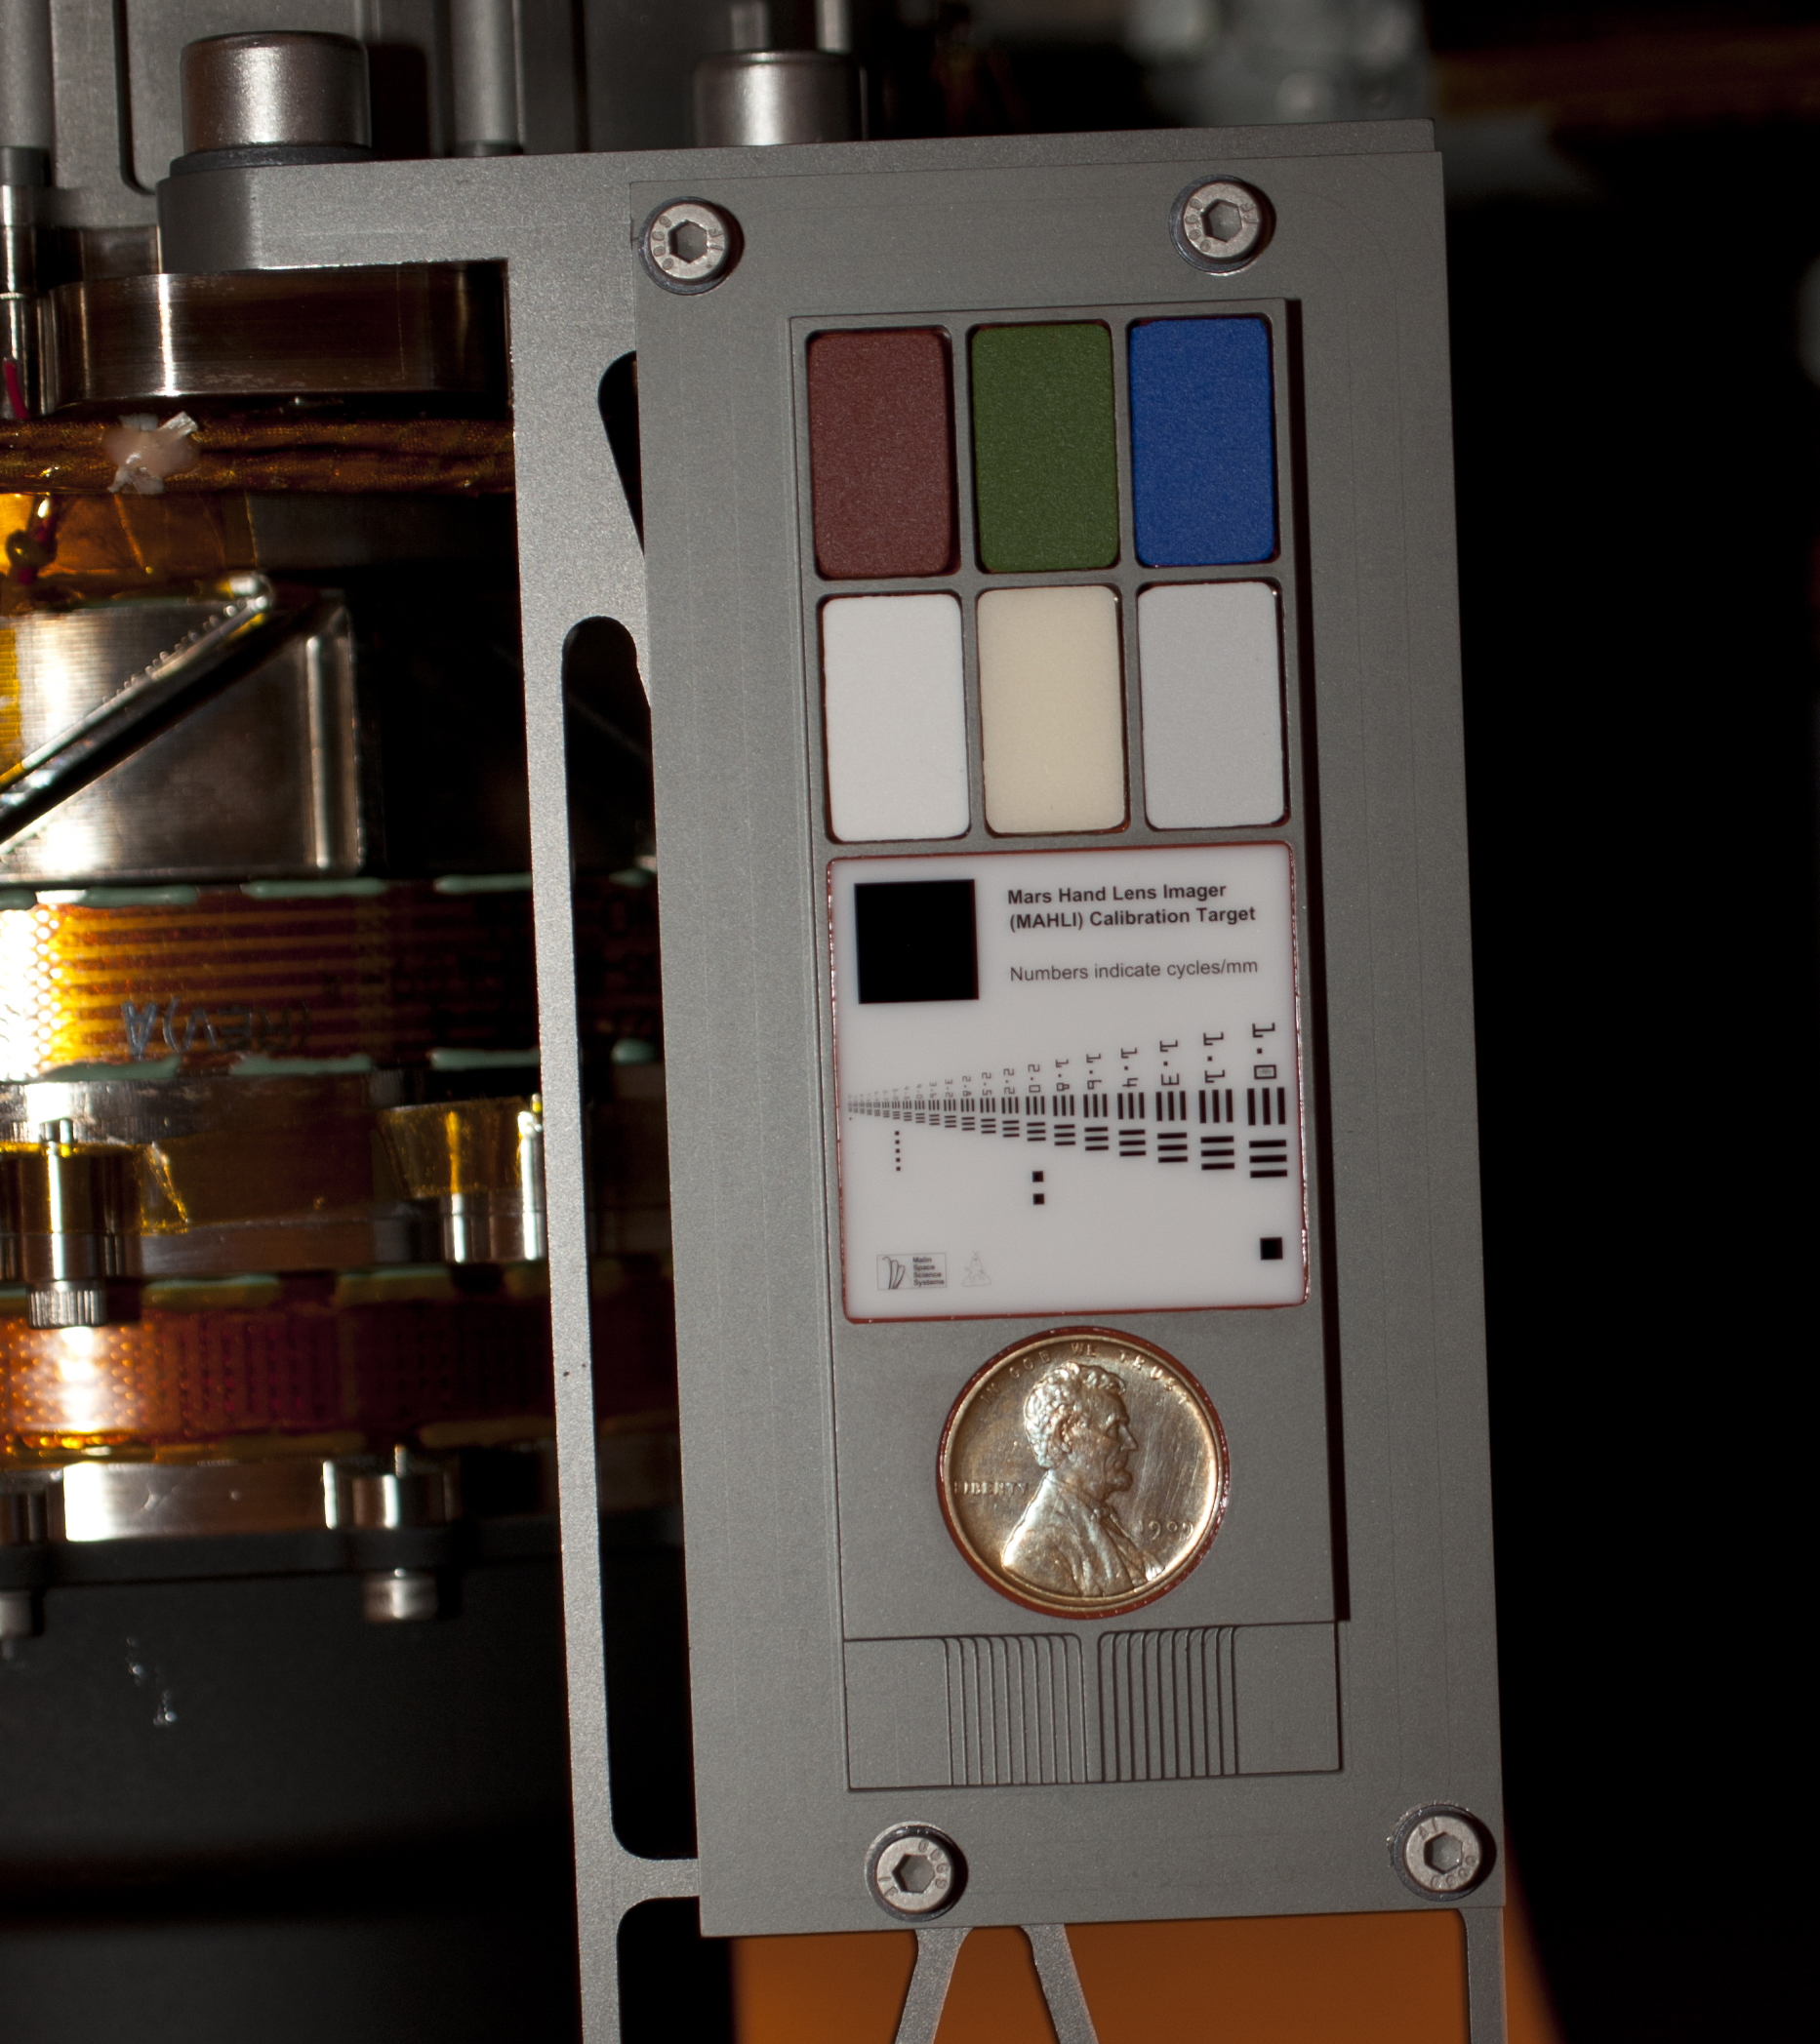
\includegraphics[width=7cm]{../images/curiosity_calibration_chart.jpg}
		\caption{The camera calibration items attached to the mars rover, Curiosity}
		\label{fig:curiosity_calibration_chart}
	\end{figure} 